We will present a calculus with special constructions for dealing with
effects and handlers, which we will then apply to the problem of natural
language semantics in the rest of the thesis. Our calculus is an extension
of the simply-typed lambda calculus (STLC). We enrich STLC with a type for
representing effectful computations alongside with operations to create and
process values of this type.

\chapter{Definitions}
\label{ch:definitions}

We are tempted to start by first giving the formal definitions of all the
essential components of our calculus:

\begin{itemize}
\item the syntax of the terms in our calculus
\item the syntax of the types in our calculus
\item the judgments that relate types to terms
\item a reduction semantics
\end{itemize}

However, before we do so, we will briefly sketch the ideas behind the
calculus so you can start building an intuition about the meaning of the
symbols that we will be introducing below.

\section{Sketching Out the Calculus}
%% \todo{This now serves both as a sketch and a justification of the calculus,
%%   along with the history of the techniques used. This could maybe later
%%   live in its own place, somewhere in the introduction.}

We will be adding a new type constructor, $\FF$, into our
language. The type $\FF(\alpha)$ will correspond to effectful
\emph{computations} that produce values of type $\alpha$. The idea comes
from the programming language Haskell and its use of monads
\cite{moggi1991notions,wadler1992essence,jones2003haskell}. Our type
constructor $\FF$ will also stand in for a monad, one that has been
already encoded in Haskell in several ways
\cite{kiselyov2013extensible,kammar2013handlers}. The motivation behind our
calculus is thus to build a minimal language which gives us directly the
primitive operations for working with this particular monad. This way, we
end up with a language that:
\begin{itemize}
\item is smaller than Haskell (and thus more mananageable to analyse),
\item is closer to the STLC favored by semanticists,
\item and which makes more evident the features that our proposal relies on.
\end{itemize}

The transition from type $\alpha$ to a type $\FF(\alpha)$ is meant
as a generalization of a scheme often seen in semantics when novel forms of
meaning are studied (e.g., type raising \cite{montague1973proper},
dynamization \cite{lebedeva2012expression}, intensionalization
\cite{de2013note}). The distinction between the type $\alpha$ and the type
$\FF(\alpha)$ will, in different analyses, align with dichotomies
such as the following:

\begin{itemize}
\item reference/sense
\item static/dynamic meaning
\item extension/intension
\item semantics/pragmatics
\end{itemize}

The question then is, what form should our general $\FF$ type
constructor take? We want to have a construction that can combine all the
existing ones. One can do the combining at the level of monads with the use
of monad transformers, a technique pioneered by Moggi and very
well-established in the Haskell programming community
\cite{moggi1991notions}. Simon Charlow has made the case that this
technique can be exploited to great benefit in natural language semantics
as well \cite{charlow2014semantics}.

However, a competing technique has emerged in recent years and it is the
goal of this thesis to introduce it to semanticists and verify its
applicability to the study of natural language. The technique goes by many
names, ``algebraic effects and handlers'' and ``extensible effects'' being
the most commonly used ones. This is in part due to the fact that it lies
at the confluence of several research programs. This fact will allow us to
present the theory from two different perspectives so you can be equipped
with two different intuitive models.

%% Mention Lewis' ``What should meanings do instead of what should meanings
%% be.'' somewhere?

\subsubsection*{Algebraic Effects and Handlers}

Hyland, Power and Plotkin have studied the problem of deriving denotational
semantics of programming languages that combine different side effects
\cite{hyland2006combining}. In their approach, rather then modeling the
individual effects using monads and combining the monads, every effect is
expressed in terms of \emph{operators} on computations. Computations thus
become algebraic expressions with effects as operations and values as part
of the generator set.

Let us take the example of nondeterminism. In the monadic framework, this
effect is analyzed by shifting the type of denotations from $\alpha$ to the
powerset $\PP(\alpha)$. In the algebraic framework, a binary
operator $+$ is introduced and is given meaning through a set of equations.
In this case, these are the equations of a semilattice (stating the
operator's associativity, commutativity and idempotence).

When the time comes to combine two effects, their signatures are summed
together and their theories are combined through either a sum or a tensor
(a sum that adds commutativity laws for operators coming from the two
different effects).

In order to fit exception handlers into their theory, Plotkin and Pretnar
enriched the theory with a general notion of a \emph{handler}
\cite{plotkin2013handling}. A handler's purpose is to replace occurrences
of an operator within a computation by another expression. This notion was
shown to be very useful. Since using a handler on a computation is similar
to interpreting its algebraic expression in a particular algebra, in many
practical applications, the use of handlers has replaced equational
theories altogether
\cite{bauer2012programming,kammar2013handlers,brady2013programming}.

\subsubsection*{Extensible Effects}

In the early 90's, Cartwright and Felleisen were working on the following
problem. Imagine you have a simple programming language along with some
denotational semantics or some other interpretation. In your simple
language, numerical expressions might be interpreted as numbers. In that
case, the literal number 3 would denote the number 3 and the application of
the sum operator to two numerical expressions would denote the sum of their
interpretations. Now consider that you want to add mutable variables to
your language. Numerical expressions no longer denote specific numbers, but
rather functions from states of the variable store to both a number and an
updated variable store (since expressions can now both read from and write
to variables). The number 3 is thus no longer interpreted as the number 3
but as a combination of a constant function yielding the number 3 and an
identity function. The addition operator now has to take care to thread the
state of the memory through the evaluation of both of its arguments. In
short, we are forced to give new interpretations for the entire language.

Cartwright and Felleisen proposed a solution to this problem
\cite{cartwright1994extensible}. In their system, an expression can either
yield a value or produce an effect. If it produces an effect, the effect
percolates through the program all the way to the top, with the context
that the effect projected from stored as a continuation. The effect and the
continuation are then passed to an external ``authority'' that handles the
effect, often by producing some output and passing it back to the
continuation. When a new feature is added to the language, it often
suffices to add a new kind of effect and introduce a new clause into the
central ``authority''. The central authority then ends up being a
collection of small modular interpreters for the various effect
types. Denotation-wise, every expression can thus have a stable denotation
which is either a pure value or an effect request coupled with a
continuation.

Later on, this project was picked up by Oleg Kiselyov, who, following
Plotkin and Pretnar's work on handlers, proposed to break down the
``authority'' into the smaller constituent interpreters and have them be
part of the language themselves \cite{kiselyov2013extensible}.

\subsubsection*{Synthesis}

In our language, we can see values of type $\FF(\alpha)$ as
algebraic expressions built on top of some effect signature and the
generator set $\alpha$. Since an
%% \todo{Maybe introduce a more precise term
%%   which would correspond to an algebraic expression in which variables have
%%   been replaced by members of a carrier/generator set.}
{algebraic expression} is either a constant or an operator applied to some
other expressions/computations, we can also use the ``extensible effects''
perspective. Under that perspective, we can think of computations as
something which is either a pure value or an effect coupled with a
continuation (the effect corresponds to the operator and the continuation
to the indexed family of operands).

Our calculus will contain tools for injecting values of type $\alpha$ into
the type of algebraic expressions $\FF(\alpha)$, as well as tools
for constructing expressions using operators from the effect
signature. Under the ``extensible effects'' point of view, the latter can
be seen as tools for creating a computation that will raise a request to
perform an effect.

Finally, we will have a special form for defining handlers. In the
``algebraic effects and handlers'' frame of mind, these can be thought of
folds or catamorphisms that traverse the algebraic expression and transform
certain operators within. On the other hand, with ``extensible effects'',
the intuition is more similar to that of an exception handler which
intercepts requests of a certain type and decides how the computation
should continue.

\section{Terms}

Having sketched the idea behind our calculus, we will now turn our
attention to the specifics. We start by defining the syntactic
constructions used to build the terms of our language.

Without further ado, we give the syntax of the expressions of our
language. First off, let $\XX$ be a set of variables, $\Sigma$ a typed
signature and $\EE$ a set of operation symbols.

The expressions of our language are comprised of the following:
\begin{description}
  \item[abstraction] $\lam{x}{M}$, where $x$ is a variable from $\XX$ and
    $M$ is an expression
  \item[application] $\ap{M}{N}$, where $M$ and $N$ are expressions
  \item[variable] $x$, where $x$ is a variable from $\XX$
  \item[constant] $c$, where $c$ is a constant from $\Sigma$
  \item[operation] $\op{op}$, where $\op{op}$ is an operator from $\EE$
  \item[injection] $\eta$
  \item[handler] $\cdbanana$
    where $\op{op}_i$ are operators from $\EE$ and $M_i$ and $M_\eta$ are
    expressions
  \item[extraction] $\cherry$
  \item[exchange] $\CC$
\end{description}

The first four constructions --- abstraction, application, variables and
constants --- come directly from STLC with constants.

The next four deal with the algebraic expressions used to encode
computations. Let us sketch the behaviors of these four kinds of
expressions under the two readings outlined above.

\subsection*{Algebraic Expressions -- The Denotational View}

The $\eta$ function serves to inject values from the generator set into the
set of algebraic expressions. It is a constructor for the trivial atomic
algebraic expression consisting of just a single constant.

Next, for every symbol $\op{op}$ in $\EE$, we have a corresponding function
$\op{op}$ in our calculus. The function $\op{op}$ is a constructor for
algebraic expressions whose topmost operation is $\op{op}$. The $\op{op}$
constructor takes as argument a function that provides its operands, which
are further algebraic expressions.

The banana brackets $\cdbanana$ contain algebras: interpretations of
operators and constants. These components are combined into a catamorphism
that can interpret algebraic expressions (hence the use of banana brackets
\cite{meijer1991functional})\footnote{Since the banana brackets can contain
  an arbitrary number of operator clauses, we use the syntax of named
  parameters/records commonly used in popular programming languages such as
  Ruby, Python or JavaScript.}.

The extraction function $\cherry$, pronounced ``cherry'', takes an atomic
algebraic expression (the kind produced by $\eta$) and projects out the
element of the generator set.

\subsection*{Effectful Computations -- The Operational View}

We will now explain these constructions from the computational point of
view.

The $\eta$ function ``returns'' a given value. The result of applying it to
a value $x$ is a computation that immediately terminates and produces the
value $x$.

The symbols from $\EE$ become something like system calls. A computation
can interrupt its execution and throw an exception with a request to
perform a system-level operation. For every symbol $\op{op}$ in $\EE$,
there is a constructor $\op{op}$ that produces a computation which issues a
request to perform the operation $\op{op}$. This constructor takes as an
argument a continuation which yields the computation that should be pursued
after the system-level operation $\op{op}$ has been performed.

The banana brackets $\cdbanana$ describe handlers: they contain clauses for
different kinds of interrupts (operation requests) and for successful
computations (clause $\eta$). They behave very much like handlers in
languages with resumable exceptions such as Common Lisp or Dylan.

Finally, the cherry function $\cherry$ can take a computation that is
guaranteed to be free of side effects and run it to capture its result.

\vspace{2em}

The 9th construction in our calculus is the $\CC$ operator. $\CC$ serves as
a link between the function type discussed by STLC (constructions 1--4) and
the computation type introduced in our calculus (constructions 5--8). $\CC$
is a (partial) function that takes a computation that produces a function
and returns a function that yields computations. In a way, $\CC$ makes
abstracting over a variable and performing an operation commute
together\footnote{This is \emph{very} reminiscent of the idea behind Paul
  Blain Levy's call-by-push-value calculus \cite{levy1999call}, which
  treats abstracting over a variable as an effectful operation of popping a
  value from a stack. Using call-by-push-value should prove to be a
  rewarding way to refine our approach.}.

We will see the utility of $\CC$ later on. The idea came to us from a paper
by Philippe de Groote \cite{degroote2015conservativity} which tried to
solve a similar problem. The name comes from the $\mathbf{C}$ combinator,
which reorders the order of abstractions in a $\lambda$-term. $\mathbf{C}$
can be seen as a special case of our $\CC$ when the type of computations
producing values $\alpha$ is $\gamma \to \alpha$ for some $\gamma$.


\section{Types and Typing Rules}
\label{sec:types}

We now give a syntax for the types of our calculus alongside with a typing
relation. In the grammar below, $\nu$ ranges over atomic types from set
$\TT$.

The types of our language consist of:
\begin{description}
\item[function] $\alpha \to \beta$, where $\alpha$ and $\beta$ are types
\item[atom] $\nu$, where $\nu$ is an atomic type from $\TT$
\item[computation] $\FF_E(\alpha)$, where $\alpha$ is a type and $E$ is an
  effect signature (defined next)
\end{description}

The only novelty here is the $\FF_E(\alpha)$
computation\footnote{Throughout this manuscript, we will be using the term
  \emph{computation} to mean values of type $\FF_E(\alpha)$. Programs
  written in our calculus are simply called terms and their normal forms
  are called values. To break it down, in our calculus, terms evaluate to
  values, some of which can be computations (those of an $\FF$ type).}
type. This type will be inhabited by effectful computations that have
permission to perform the effects described in $E$ and yield values of type
$\alpha$. The representation will be that of an algebraic expression with
operators taken from the signature $E$ and constants (elements of the
generator set) taken to be in type $\alpha$.

In giving the typing rules, we will rely on the standard notion of a
\emph{context}. For us, specifically, a context is a partial mapping from
the variables in $\XX$ to the types defined above.  We commonly write
$\Gamma, x : \alpha$ for a context that assigns to $x$ the type $\alpha$
and to other variables $y$ the type $\Gamma(y)$. We also write $x : \alpha
\in \Gamma$ to say that the context maps $x$ to $\alpha$. Note, however,
that for $\Delta = \Gamma, x : \alpha, x : \beta$, $x : \beta \in \Delta$
while $x : \alpha \notin \Delta$.

\emph{Effect signatures} are very much like contexts. They are partial
mappings from the set of operation symbols $\EE$ to pairs of types. We will
write the elements of effect signatures the following way:
$\typedop{op}{\alpha}{\beta} \in E$ means that $E$ maps $\op{op}$ to the
pair of types $\alpha$ and $\beta$\footnote{The two types $\alpha$ and
  $\beta$ are to be seen as the operation's \emph{input} and \emph{output}
  types, respectively.}. When dealing with effect signatures, we will often
make use of the disjoint union operator $\uplus$. The term $E_1 \uplus E_2$
serves as a constraint demanding that the domains of $E_1$ and $E_2$ be
disjoint and at the same time it denotes the effect signature that is the
union of $E_1$ and $E_2$.

The last kind of dictionary used by the type system is a standard
\emph{higher-order signature} for the constants (a map from names of
constants to types). For those, we adopt the same conventions.

In our typing judgments, contexts will appear to the left of the turnstile
and they will hold information about the \emph{statically} (lexically)
bound variables, as in STLC.\@ Effect signatures will appear as indices of
computation types and they will hold information about the operations that
are \emph{dynamically} bound by handlers. Finally, there will be a single
higher-order signature that will globally characterize all the available
constants.

The typing judgments are presented in Figure~\ref{fig:types}. Metavariables
$M$, $N$\ldots\ stand for expressions, $\alpha$, $\beta$,
$\gamma$\ldots\ stand for types, $\Gamma$, $\Delta$\ldots\ stand for
contexts, $\op{op}$, $\op{op}_i$ stand for operation symbols and $E$,
$E'$\ldots\ stand for effect signatures. $\Sigma$ refers to the
higher-order signature giving types to constants.

\newcommand{\handlerrule}{
 \begin{prooftree}
  \AxiomC{$E = \{\typedopg{\op{op}_i}{\alpha_i}{\beta_i}\}_{i \in I} \uplus E_f$}
  \noLine
  \def\extraVskip{0pt}
  \UnaryInfC{$E' = E'' \uplus E_f$}
  \noLine
  \UnaryInfC{$[\Gamma \vdash M_i : \alpha_i \to (\beta_i \to
    \FF_{E'}(\delta)) \to \FF_{E'}(\delta)]_{i \in I}$}
  \noLine
  \UnaryInfC{$\Gamma \vdash M_\eta : \gamma \to \FF_{E'}(\delta)$}
  \def\extraVskip{2pt}
  \RightLabel{[$\banana{}$]}
  \UnaryInfC{$\Gamma \vdash \cibanana : \FF_{E}(\gamma) \to \FF_{E'}(\delta)$}
 \end{prooftree}}

\begin{figure}
  \def\labelSpacing{4pt}

  \begin{subfigure}{.5\textwidth}
   \begin{prooftree}
    \AxiomC{$\Gamma, x : \alpha \vdash M : \beta$}
    \RightLabel{[abs]}
    \UnaryInfC{$\Gamma \vdash \lam{x}{M} : \alpha \to \beta$}
   \end{prooftree}
  \end{subfigure}
  \begin{subfigure}{.5\textwidth}
   \begin{prooftree}
    \AxiomC{$\Gamma \vdash M : \alpha \to \beta$}
    \AxiomC{$\Gamma \vdash N : \alpha$}
    \RightLabel{[app]}
    \BinaryInfC{$\Gamma \vdash M N : \beta$}
   \end{prooftree}
  \end{subfigure}

  \vspace{2mm}
 
  \begin{subfigure}{.5\textwidth}
   \begin{prooftree}
    \AxiomC{$x : \alpha \in \Gamma$}
    \RightLabel{[var]}
    \UnaryInfC{$\Gamma \vdash x : \alpha$}
   \end{prooftree}
  \end{subfigure}
  \begin{subfigure}{.5\textwidth}
   \begin{prooftree}
    \AxiomC{$c : \alpha \in \Sigma$}
    \RightLabel{[const]}
    \UnaryInfC{$\Gamma \vdash c : \alpha$}
   \end{prooftree}
  \end{subfigure}

  \vspace{6mm}

  \begin{subfigure}{.5\textwidth}
   \begin{prooftree}
    \AxiomC{$\Gamma \vdash \eta : \alpha \to \FF_E(\alpha)$
    \hskip 4pt [$\eta$]}
   \end{prooftree}
  \end{subfigure}
  \begin{subfigure}{.5\textwidth}
   \begin{prooftree}
    \AxiomC{$\Gamma \vdash \cherry : \FF_\emptyset(\alpha) \to \alpha$
    \hskip 4pt [$\cherry$]}
   \end{prooftree}
  \end{subfigure}

  \vspace{3mm}

  \hspace{-1.5cm}
  \begin{subfigure}{.5\textwidth}
   \begin{prooftree}
    \AxiomC{$\typedop{op}{\alpha}{\beta} \in E$}
    \RightLabel{[op]}
    \UnaryInfC{$\Gamma \vdash \op{op} : \alpha \to (\beta \to \FF_E(\gamma)) \to \FF_E(\gamma)$}
   \end{prooftree}
  \end{subfigure}
  \hspace{1cm}
  \begin{subfigure}{.5\textwidth}
   \handlerrule
  \end{subfigure}

  \vspace{6mm}

  \begin{subfigure}{\textwidth}
   \begin{prooftree}
    \AxiomC{$\Gamma \vdash \CC : (\alpha \to \FF_E(\beta)) \to
      \FF_E(\alpha \to \beta)$
    \hskip 4pt [$\CC$]}
   \end{prooftree}
  \end{subfigure}

  \caption{\label{fig:types}Typing rules for our calculus.}
\end{figure}


The typing rules mirror the syntax of expressions. Again, the first four
rules come from STLC.\@ The next four deal with introducing pure
computations, enriching them with effectful operations, handling those
operations away and finally eliminating pure computations. The $\CC$ rule
lets us start to see what we meant by saying that the $\CC$ operator lets
the function type and the computation type commute.

Let us ponder the types of the new constructions so as to get a grip on the
interface that the calculus provides us for dealing with computation
values.

\subsection*{[$\eta$]}

First off, we have the $\eta$ operator. It takes a value of type $\alpha$
and injects it into the type $\FF_E(\alpha)$. The meta-variable $E$ is
free, meaning $\eta$ can take values of type $\alpha$ to type
$\FF_E(\alpha)$ for any $E$. The algebraic intuition would say that elements
of the generator set are valid algebraic expressions independent of the
choice of signature. Computationally, returning a value is always an
option, independently of the available permissions.

\subsection*{[op]}

More complicated computations can be built up by extending existing
computations using the \textbf{operation} construction. Let us have an
effect signature $E$, such that $\typedop{op}{\alpha}{\beta} \in E$. To use
$\op{op}$, we first apply it to a value of the input type $\alpha$ and to a
continuation. The continuation is a function of type $\beta \to
\FF_E(\gamma)$ that accepts a value of the output type $\beta$ (the result
of performing the operation) and chooses in return a computation that
should be pursued next. The return type of our new computation will thus be
the return type $\gamma$ of the computation provided by the
continuation. The continuation's computation and the new extended
computation will also share the same effect signature $E$. This means that
all uses of the operation $\op{op}$ within the created computation have the
same input and output types\footnote{In general, the same operation symbol
  can be used in different computations whose types are indexed by
  different effect signatures.}.

Notice also how the [op] rule is similar to the [var] rule in that it lets
use a symbol with a certain type given that it exists in some kind of
signature/context. The crucial difference is that contexts are components
of judgments whereas effect signatures are components of types. The meaning
of a variable is determined by inspecting the expression in which it occurs
and finding the $\lambda$ that binds it (this is known as \emph{lexical} or
\emph{static binding}). On the other hand, the meaning of an operation in a
computation is determined by evaluating the term in which the computation
appears until the computation becomes the argument of a handler. This
handler will then give meaning to the operation symbol by effectively
substituting it with a suitable interpretation (this kind of \emph{late}
binding is known as \emph{dynamic binding}).

We have now seen how to construct pure computations using $\eta$ and extend
them by adding operations. However, before we go on and start talking about
handlers, we would like to give the algebraic intuition behind [op], as the
algebraic point of view makes explaining the handler rule [$\banana{}$]
easier.

We can see the effect signature as an algebraic signature. Whenever we have
$\typedop{op}{\alpha}{\beta} \in E$, we have an $\alpha$-indexed family of
operators of arity $\beta$. Let's unpack this statement.

\begin{itemize}
\item First, there is the matter of having an indexed family of
  operators. A common example of these is the case of scalar multiplication
  in the algebra of a vector space. A \emph{single-sorted algebraic
    signature} is a set of operation symbols, each of which is given an
  arity (a natural number). For vector addition, the arity is 2, since
  vector addition acts on two vectors (two elements of the
  domain). Scalar multiplication acts on one scalar and one
  vector. However, neither arity 1 nor arity 2 adequately express this. We
  can get around the limitations of a single-sorted signature by
  introducing for every scalar $k$ an operation of arity 1 that corresponds
  to multiplying the vector by $k$. Scalar multiplication is therefore not
  a single operator but a scalar-indexed family of operators.

  The very same strategy is applied here as well. A single operation symbol
  doesn't need to map to a single operator but can instead map to (possibly
  infinitely) many operators indexed by values of some type $\alpha$. For
  example, writing messages to the program's output
  ($\typedop{print}{string}{1}$) can be seen as a string-indexed family of
  unary operators on computations. For every string $s$, we get an operator
  that maps computations $c$ to computations that first print $s$ and then
  continue as $c$.

\item Next, we were speaking about operators of arity $\beta$. The use of a
  type in place of a numerical arity is due to a certain generalization. In
  set theory, natural numbers become sets that have the same cardinality as
  the number they represent ($\left\vert N \right\vert = N$). We can
  therefore conservatively generalize the idea of arity to a set by saying
  that an operator of arity $X$ takes one operand per each element of the
  set $X$. It's a short step from there to using types as arities, wherein
  an operator of arity $\beta$ takes one operand per possible value of type
  $\beta$.

  This will come in very handy in our system. We want our operator
  $\op{op}$ to have as many operands as there are possible values in the
  output type $\beta$. Therefore, we simply say that the operator has arity
  $\beta$.

  How do we write down the application of an operator of arity $\beta$ to
  its operands? We can no longer just list out all the operands, since
  types in our calculus may have an unbounded number of inhabitants. We
  will organize operands in \emph{operand clusters}\footnote{Our use of the
  word \emph{cluster} is synonymous with the mathematical term
  \emph{family}. We will be using the term \emph{cluster} for families of
  computations passed to operations and handlers.}, arity-indexed families
  of operands. We will write them down as functions, using
  $\lambda$-abstraction, from the arity type $\beta$ to some operand type,
  e.g., $\FF_E(\gamma)$.
\end{itemize}

Now we can understand what it means to say that
$\typedop{op}{\alpha}{\beta} \in E$ gives rise to an $\alpha$-indexed
family of operators of arity $\beta$. We apply to $\op{op}$ an index of
type $\alpha$ to get an operator and then we apply that operator to an
operand cluster of type $\beta \to \FF_E(\gamma)$ to get a new expression
of type $\FF_E(\gamma)$.

We suggest visualizing these algebraic expressions as trees (see Section~2
of \cite{lindley2014algebraic} for the original idea). Trees of type
$\FF_E(\alpha)$ consist of leafs containing values of type $\alpha$ and
internal nodes labelled with operations and their parameters. Every
internal node is labelled with some $\typedop{op}{\alpha}{\beta} \in E$ and
with a parameter of type $\alpha$ and it has a cluster of children indexed
by $\beta$.

\subsection*{[$\banana{}$]}

Now we are ready to explain the handler rule. Let us have some computation
$N : \FF_E(\gamma)$ (which we can now think of as an algebraic expression
or a tree). By applying the handler $\cibanana$ to $N$, we get a new
computation $N' : \FF_{E'}(\delta)$. The typing rule for $\banana{}$ is
repeated in Figure~\ref{fig:handler-rule}.

\begin{figure}
  \handlerrule
  \caption{\label{fig:handler-rule} The typing rule for the handler
    construction.}
\end{figure}

To illustrate the constraints on the types of the components, $M_i$ and
$M_\eta$, of a handler, we will examine its semantics. The handler
processes the tree $N$ by recursive induction. Depending on the shape of
the tree, one of the following will happen:

\begin{itemize}
\item If $N$ is a leaf, then the value stored in the leaf is of type
  $\gamma$. This is where the $M_\eta$ function comes in. It must take a
  value of type $\gamma$ and produce a new tree of type $\FF_{E'}(\delta)$,
  hence the fourth hypothesis of the $\banana{}$ rule.

\item If $N$ is an internal node labelled with the operation symbol
  $\op{op}_i$ for some $i \in I$ and some parameter, then that parameter
  must be of type $\alpha_i$. Furthermore, this node will have a
  $\beta_i$-indexed cluster of children. We know this since $N$ is of type
  $\FF_E(\gamma)$ and the first hypothesis tells us that
  $\typedopg{\op{op}_i}{\alpha_i}{\beta_i} \in E$.

  We will recursively apply our handler to the cluster of children,
  changing their type from $\FF_E(\gamma)$ to $\FF_{E'}(\delta)$. We now
  need something which takes the parameter in the node, type $\alpha_i$,
  and the family of the processed subtrees, type $\beta_i \to
  \FF_{E'}(\delta)$, which is exactly the function $M_i$ in the third
  hypothesis of the $\banana{}$ rule.

\item If $N$ is an internal node labelled with some operation symbol
  $\op{op}$ such that $\typedop{op}{\alpha}{\beta} \in E_f$ for some
  $\alpha$ and $\beta$, then we will ignore the node and process only its
  children. This means that the resulting tree will contain the operation
  $\op{op}$ and any other symbols defined in $E_f$\footnote{The $f$ in
    $E_f$ stands for \emph{forwarded effects}, since it refers to effects
    that the handler will not interpret but instead forward to some other
    interpreter.}. In order for such a tree to be of the desired type
  $\FF_{E'}(\delta)$, $E_f$ must be a subset of $E'$, which is what the
  second hypothesis of the $\banana{}$ rule guarantees.
\end{itemize}

We have covered the whole $\banana{}$ rule, except for the presence of the
effect signature $E''$. It serves two roles.

\begin{itemize}
\item First of all, it acts as a ``free'' variable over effect
  signatures. This means that we can give any effect signature $E'$ to the
  type $\FF_{E'}(\delta)$ of the resulting computation $N'$ as long as $E'$
  contains $E_f$ ($E''$ represents the relative complement of $E_f$ in
  $E'$). This is in analogy to the free effect variable $E$ in the [$\eta$]
  and [op] rules. This freedom of effect variables is a way of implementing
  the idea that a computation of type $\FF_{E_1}(\alpha)$ can be used
  anywhere that a computation of type $\FF_{E_2}(\alpha)$ given that $E_1
  \subseteq E_2$\footnote{This relation is an instance of subtyping and a
    more robust treatment will be outlined in Section~\ref{sec:subtyping}.}.

\item In the previous paragraph, why did we put the word ``free'' in
  quotation marks?  Because the effect variable $E''$ is not actually
  free. It is the complement of $E_f$ in $E'$ and $E'$ is constrained by
  the types of $M_i$ and $M_\eta$ in the third and fourth hypotheses,
  respectively. The handler's clauses might themselves introduce new
  effects, which will in turn translate into constraints on $E'$ and
  $E''$. This happens when a handler interprets an operation by making an
  appeal to some other operation (e.g.\ a handler can interpret
  computations using n-ary choice into computation using binary choice).

  As the simplest example, we can take a handler that replaces one
  operation symbol with another,
  $\banana{\onto{\op{old}} \op{new},\ \onto{\eta} \eta}$. The type scheme
  corresponding to the term is $\FF_{\{\typedop{old}{\alpha}{\beta}\}
    \uplus E_f}(\gamma) \to \FF_{\{\typedop{new}{\alpha}{\beta}\} \uplus
    E^3 \uplus E_f}(\gamma)$. In this scheme, $\alpha$, $\beta$ and
  $\gamma$ are free meta-variables ranging over types and $E_f$ and $E^3$
  are free over effect signatures. The $E''$ of the $\banana{}$ rule
  corresponds to $\{\typedop{new}{\alpha}{\beta}\} \uplus E^3$. The handler
  has eliminated the $\op{old}$ effect but it has also introduced the
  $\op{new}$ effect.
\end{itemize}

This concludes our exploration of the $\banana{}$ rule. We have explained
it in terms of algebraic expressions and trees, using the denotational
intution. We will develop the operational intuition, which talks about
handlers in terms of computations and continuations, in
Section~\ref{sec:reductions}, where we will give the semantics of our
language using reduction rules.

\subsection*{[cherry]}

Next up is the cherry operator, $\cherry$. Its type is
$\FF_\emptyset(\alpha) \to \alpha$ and it serves as a kind of dual to the
$\eta$ opertator, an elimination for the $\FF$ type.

The type $\FF_\emptyset(\alpha)$ demands that the effect signature be
empty. In such a case, the tree has no internal nodes and is composed of
just a leaf containing a value of the type $\alpha$. The $\cherry$ operator
serves to extract that value.

Another way to look at it is to say that a computation of type
$\FF_\emptyset(\alpha)$ cannot perform any ``unsafe'' operations and it is
therefore always safe to execute it and get the resulting value of type
$\alpha$.

\subsection*{[$\CC$]}

Finally, we take a look at the $\CC$ operator. The type of the operator is
$(\alpha \to \FF_E(\beta)) \to \FF_E(\alpha \to \beta)$. Its input is an
$\alpha$-indexed family of computations and its output is a computation of
$\alpha$-indexed families. The operator applies only in the case when all
the computations in the family share the same \emph{internal structure}. By
sharing the same \emph{internal structure}, we mean that the trees can only
differ in their leaves. What the $\CC$ operator then does is to push the
$\lambda$-binder down this common internal structure into the leaves (see
Figure~\ref{fig:c-illustration} for an example). This way, we can
evaluate/handle the common operations without commiting to a specific value
of type $\alpha$.

\begin{figure}
  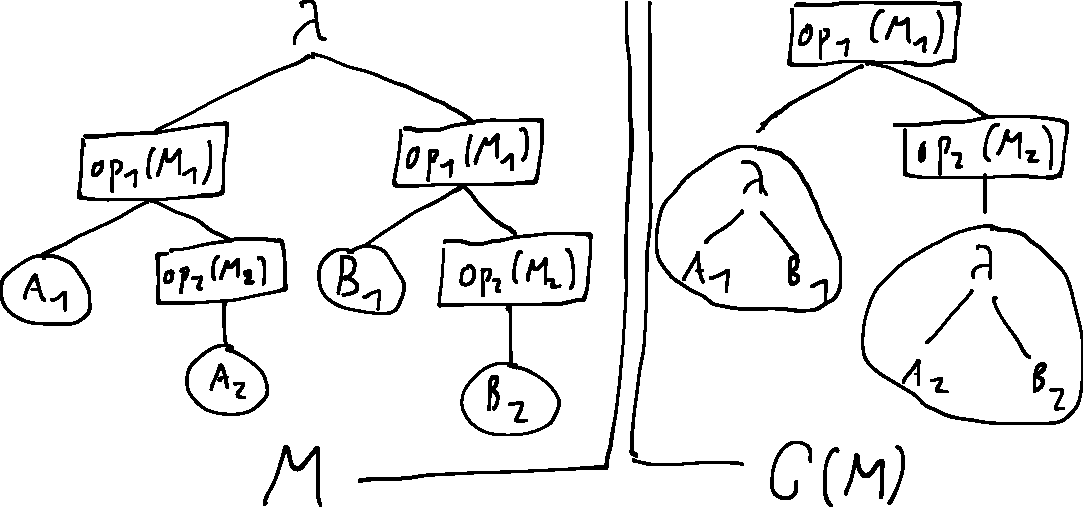
\includegraphics[width=\textwidth]{doodles/c-illustration}
  \caption{\label{fig:c-illustration} Example of applying the $\CC$
    operator to a term. Functions/families are drawn as trees. In this
    example, the $\lambda$ binds a variable of a binary type, the output of
    $\op{op}_1$ is binary and the output of $\op{op}_2$ is
    unary. \TODO{This doodle is a placeholder for a cleaner picture
      generated by a program (or at least until I learn to draw).}}
\end{figure}

We can also explain the action of $\CC$ in operational terms. As in
call-by-push-value~\cite{levy1999call}, we can think of abstraction over
$\alpha$ as some effectful operation that tries to pop a value $x : \alpha$
off a stack. The input of $\CC$ can then be seen as a continuation waiting
for this $x$ and wanting to perform some further operations. $\CC$ assumes
that the continuation performs operations independently of
$x$\footnote{Violating this assumption will yield terms which get stuck
  during evaluation (we will see the partial reduction rules in
  Section~\ref{sec:reductions}). Sam Lindley presented a refined type
  system for a similar calculus to track the use of variables
  \cite{lindley2014algebraic}. A similar refinement should be possible in
  our case as well but it would obscure the already dense type notation.}
and it can thus postpone popping $x$ off the stack until after the
operations dictated by the continuation have been evaluated. $\CC$ is thus
a kind of commutativity law for operations and abstraction (the popping of
a value off the operand stack): as long as one does not depend on the
other, it does not matter whether we first perform an operation and then
abstract over an argument or whether we do so the other way
around\footnote{The other direction, typed $\FF_E(\alpha \to \beta) \to
  (\alpha \to \FF_E(\beta))$, is already possible without introducing a
  special operator since $\FF_E$ is a functor (as we will show later).}.


\section{Reduction Rules}
\label{sec:reductions}

We will now finally give a semantics to our calculus. The semantics will be
given in the form of a reduction relation on terms. Even though the point
of the calculus is to talk about effects, the reduction semantics will have
no notion of order of evaluation or evaluation context; any subexpression
that is reducible can be reduced in any context.

Before we dive into the reduction rules proper we will first have to handle
some formal paperwork, most of it due to the fact that we use variables and
binders in our calculus. In order to quotient out the irrelevant
distinction between terms that are the same up to variable names, we will
introduce a series of definitions leading up to a notion of
$\alpha$-equivalence.

\begin{definition}
  Let $M$ be a term in our calculus. We define the set of \textbf{free
    variables} of $M$, written $\FV(M)$, using the following set of
  equations:

  \begin{align*}
    \FV(\lam{x}{M}) &= \FV(M) \setminus \{x\} \\
    \FV(\ap{M}{N}) &= \FV(M) \cup \FV(N) \\
    \FV(x) &= \{x\} \\
    \FV(c) &= \emptyset \\
    \FV(\op{op}) &= \emptyset \\
    \FV(\eta) &= \emptyset \\
    \FV(\cibanana) &= \bigcup_{i \in I} \FV(M_i) \cup \FV(M_\eta) \\
    \FV(\cherry) &= \emptyset \\
    \FV(\CC) &= \emptyset
  \end{align*}
\end{definition}

Most often, we will make use of $\FV$ indirectly, using the following
notion.

\begin{definition}
  We say that $x$ is \textbf{fresh} for $M$ iff $x \notin \FV(M)$.
\end{definition}

\begin{definition}
  Let $M$ and $N$ be terms and $x$ a variable. We define the
  \textbf{capture-avoiding substitution}\footnote{\TODO{Maybe add a small
      note for readers not aware of the capture problem? I do not expect
      people to be unfamiliar with it, but I do spend a few pages talking
      about the trouble with substitutions and variables so it might be
      worth it to have a small intro.}} of $N$ for $x$ in $M$, written as
  $\subst{M}{x}{N}$, using the following equations:

  \begin{align*}
    \subst{(\lam{x}{M})}{x}{N} &= \lam{x}{M} \\
    \subst{(\lam{y}{M})}{x}{N} &= \lam{y}{(\subst{M}{x}{N})} \textrm{ given
      that } y \neq x \textrm{ and $y$ is fresh for $N$} \\
    \subst{(\ap{M}{K})}{x}{N} &= \ap{(\subst{M}{x}{N})}{(\subst{K}{x}{N})} \\
    \subst{x}{x}{N} &= N \\
    \subst{y}{x}{N} &= y \textrm{ given that } x \neq y \\
    \subst{c}{x}{N} &= c \\
    \subst{\op{op}}{x}{N} &= \op{op} \\
    \subst{\eta}{x}{N} &= \eta \\
    \subst{\cibanana}{x}{N} &= \banana{(\onto{\op{op}_i}
      (\subst{M_i}{x}{N}))_{i \in I},\ \onto{\eta} (\subst{M_\eta}{x}{N})} \\
    \subst{\cherry}{x}{N} &= \cherry \\
    \subst{\CC}{x}{N} &= \CC
  \end{align*}

  Note that it is possible for $\subst{M}{x}{N}$ to not be defined by the
  equations above (e.g.\ $\subst{(\lam{y}{x})}{x}{y}$). In such cases, we
  say that the substitution does not exist.
\end{definition}

\begin{definition}
  Let $\sim$ be a binary relation on the terms of our calculus. We define
  the relation $\syntclos{\sim}$, called the \textbf{syntactic closure} of
  $\sim$, as the smallest relation\footnote{\TODO{Should I prove that such
    a relation is uniquely determined?}} that contains $\sim$ and satisfies
  the following conditions:

  \begin{itemize}
  \item if $M \syntclos{\sim} M'$, then $(\lam{x}{M}) \syntclos{\sim} (\lam{x}{M'})$
  \item if $M \syntclos{\sim} M'$, then $(\ap{M}{N}) \syntclos{\sim} (\ap{M'}{N})$
  \item if $N \syntclos{\sim} N'$, then $(\ap{M}{N}) \syntclos{\sim} (\ap{M}{N'})$
  \item if $M_i \syntclos{\sim} M_i'$, then $\banana{\onto{\op{op}_1}
    M_1,\ \dots,\ \onto{\op{op}_i} M_i,\ \dots,\ \onto{\op{op}_n}
    M_n,\ \onto{\eta}{M_\eta}} \syntclos{\sim} \banana{\onto{\op{op}_1}
    M_1,\ \dots,\ \onto{\op{op}_i} M_i',\ \dots,\ \onto{\op{op}_n}
    M_n,\ \onto{\eta} M_\eta}$
  \item if $M_\eta \syntclos{\sim} M_\eta'$, then
    $\cibanana \syntclos{\sim}
     \banana{(\onto{\op{op}_i}{M_i})_{i \in I},\ \onto{\eta}{M_\eta'}}$
  \end{itemize}
\end{definition}

Later on, we will define relations on the terms of our calculus that will
correspond to different transformations (such $\swap$ and the reduction
rules). The notion of syntactic closure will allow us to say that a term
can be transformed by transforming any of its parts.

\begin{definition}
  Let $\sim$ be a relation. We define the relation $\sim^*$, called the
  \textbf{reflexive-transitive closure} of $\sim$, as the smallest relation
  that contains $\sim$ and satisfies the following conditions:

  \begin{itemize}
  \item $x \sim^* x$ for any $x$ in the domain of $R$
  \item if $x \sim^* y$ and $y \sim^* z$, then $x \sim^* z$
  \end{itemize}
\end{definition}

\begin{definition}
  We define a relation called $\swap$ on the terms of our calculus as:

  \begin{itemize}
  \item $\lam{x}{M} \swap \lam{y}{(\subst{M}{x}{y})}$ given that $y \notin
    \FV(M)$ and that $\subst{M}{x}{y}$ exists

    %% \footnote{Also under the condition that $\subst{M}{x}{y}$
    %%   exists. We will not mention this proviso in further definitions.

    %%   Whenever we will try to define a relation between elements $f(X)$ and
    %%   $g(X)$, where $f$ and $g$ are partial functions, and either $f(X)$ or
    %%   $g(X)$ will not exist, then we will ignore the pair (i.e. $f(X)$ and
    %%   $g(X)$ will not enter into the relation since one of them does not
    %%   even exist).

    %%   Linguistically speaking, the presuppositions triggered by the
    %%   definite descriptions $f(X)$ and $g(X)$ in the sentence ``$f(X)$
    %%   relates to $g(X)$'' are resolved by adding an implicit conditional
    %%   ``if $f(X)$ and $g(X)$ both exist''. This handler will be specific to
    %%   the way we define relations. Dangling presuppositions in other parts
    %%   of the math should be seen as mistakes or omissions.}
    
  \end{itemize}
\end{definition}

\begin{definition}
  We define the relation of \textbf{$\alpha$-equivalence}, written as
  $=_\alpha$, to be $[\swap]^*$, i.e.\ the reflexive-transitive closure of
  the syntactic closure of the $\swap$ relation.
\end{definition}

\begin{observation}
  $=_\alpha$ is an equivalence relation.
\end{observation}
\begin{proof}
  $\swap$ is a symmetric relation and both syntactic closure and
  reflexive-transitive closure preserve symmetricity. Reflexivity and
  transitivity are guaranteed by the reflexive-transitive closure.
\end{proof}

The notion of $\alpha$-equivalence will be very useful. We will use it so
much that we will actually quotient the set of terms and start talking
about $\alpha$-equivalence classes instead of specific terms. We will keep
using the same notation and so from now on, terms written in the syntax of
our calculus no longer designate individual terms but rather
$\alpha$-equivalence classes of terms. The term ``term'' will itself be
freely used to actually mean an $\alpha$-equivalence class of terms.

However, before we start using individual terms while having them represent
entire $\alpha$-equivalence classes, we should better make sure that the
operations that we will perform with these terms are congruent with
$\alpha$-equivalence\footnote{Congruence means that equivalent inputs are
  mapped to equivalent outputs.}. Is it the case that the operations we
have introduced in this section are congruent with $\alpha$-equivalence?

$\FV$ is congruent: swapping names bound by $\lambda$ does not change the
set of free variables in a term.

The definition of syntactic closure works for $\alpha$-equivalence classes
as well.

What about substitution? As we have already seen, capture-avoiding
substitution is a partial operation: $\subst{(\lam{y}{x})}{x}{y}$ does not
exist. However, $\lam{z}{x}$ is $\alpha$-equivalent to $\lam{y}{x}$ and
$\subst{(\lam{z}{x})}{x}{y}$ exists; it is $\lam{z}{y}$. Not congruent.

We will introduce an alternative notion, \emph{capture-resolving
  substitution}. While capture-avoiding substitution was a partial function
on terms, capture-resolving substitution will be a total function on
$\alpha$-equivalence classes. Furthermore, the new function will be an
extension of the old one. If capture-avoiding substitution would have
mapped $A$ to $B$, then capture-resolving substitution will map the
$=_\alpha$ class of $A$ to the $=_\alpha$ class of $B$.

In defining capture-resolving substitution, we will demonstrate a technique
that is made possible by the transition from single terms to $=_\alpha$
classes of terms. When we have a variable $x$ bound in a term, we can
always assume, without loss of generality, that it is distinct from another
variable $y$ (since inside our term, we can swap $x$ with any variable from
$\XX$ which is different from $y$ and end up in the same $=_\alpha$
class). By extension, we can also assume that a variable $x$ bound in some
term is fresh in some other term.

\begin{definition}
  Let $M$ and $N$ be terms and $x$ a variable. We define the
  \textbf{(capture-resolving) substitution} of $N$ for $x$ in $M$, written as
  $\subst{M}{x}{N}$\footnote{From now on, this notation will be used for
    capture-resolving substitution only.}, using the following equations:

  \begin{align*}
    \subst{(\lam{y}{M})}{x}{N} &= \lam{y}{(\subst{M}{x}{N})} \textrm{ assuming
      that } y \neq x \textrm{ and $y$ is fresh for $N$} \footnotemark \\
    \subst{(\ap{M}{K})}{x}{N} &= \ap{(\subst{M}{x}{N})}{(\subst{K}{x}{N})} \\
    \subst{x}{x}{N} &= N \\
    \subst{y}{x}{N} &= y \textrm{ given that } x \neq y \footnotemark \\
    \subst{c}{x}{N} &= c \\
    \subst{\op{op}}{x}{N} &= \op{op} \\
    \subst{\eta}{x}{N} &= \eta \\
    \subst{\cibanana}{x}{N} &= \banana{(\onto{\op{op}_i}
      (\subst{M_i}{x}{N}))_{i \in I},\ \onto{\eta} (\subst{M_\eta}{x}{N})} \\
    \subst{\cherry}{x}{N} &= \cherry \\
    \subst{\CC}{x}{N} &= \CC
  \end{align*}
\end{definition}

\addtocounter{footnote}{-1}
\footnotetext{Here, $y$ is a bound variable and we can simply \emph{assume}
  that it is different from $x$ and proceed\dots}
\stepcounter{footnote}
\footnotetext{\dots whereas here, $y$ is a free variable and therefore, we
  have to \emph{examine} whether it is different from $x$ or not.}

We are now at a point where we can easily lay down the reduction rules for
our calculus. A reduction rule $\xi$ will be a relation on terms. Most of
the time, we will deal with their syntactic closures, $[\xi]$, for which we
will also adopt the notation $\to_\xi$. We will also use the notation
$\to_{\xi_1,\dots,\xi_n}$ for the composition $\to_{\xi_n} \circ \dots
\circ \to_{\xi_1}$. The \emph{small-step semantics} of our calculus will be
given by the union of the $\to_\xi$ relations for every reduction rule
$\xi$ and we will represent it with the plain symbol $\to$. The
\emph{big-step semantics} will be $\to^*$, the reflexive-transitive closure
of $\to$, with its codomain restricted to normal forms and we will write it
down using the symbol $\tto$. A \emph{normal form} is defined as a term $M$
for which there exists no other term $N$ such that $M \to N$.

We will now go through the reduction rules of our calculus, presented in
Figure~\ref{fig:reductions}, one by one.


\begin{figure}
  \centering
  \begin{tabular}{lr}
  $\ap{(\lam{x}{M})}{N} \to$ & rule $\beta.\to$ \\
  $\subst{M}{x}{N}$ & \\
  \\
  $\lam{x}{\ap{M}{x}} \to$ & rule $\eta.\to$ \\
  $M$ & where $x$ is fresh for $M$ \\
  \\
  $\ap{\cibanana}{(\ap{\eta}{N})} \to$ & rule $\banana{\eta}$ \\
  $\ap{M_\eta}{N}$ & \\
  \\
  $\ap{\cibanana}{(\ap{\ap{\op{op}_i}{N_p}}{N_c})} \to$ & rule $\banana{\op{op}}$ \\
  $\ap{M_i}{\ap{N_p}{(\lam{x}{\ap{\cibanana}{(\ap{N_c}{x})}})}}$
  & where $x$ is fresh for $M_\eta$ \\ & and $M_i$ for all $i \in I$ \\
  \\
  $\ap{\cibanana}{(\ap{\ap{\op{op}'}{N_p}}{N_c})} \to$ & rule $\banana{\op{op}'}$ \\
  $\ap{\op{op}'}{\ap{N_p}{(\lam{x}{\ap{\cibanana}{(\ap{N_c}{x})}})}}$
  & where $\op{op}' \notin \{\op{op}_i\}_{i \in I}$ \\
  & and $x$ is fresh for $M_\eta$ \\ & and $M_i$ for all $i \in I$ \\
  \\
  $\ap{\cherry}{(\ap{\eta}{M})} \to$ & rule $\cherry$ \\
  $M$ & \\
  \\
  $\ap{\CC}{(\lam{x}{\ap{\eta}{M}})} \to$ & rule $\CC_\eta$ \\
  $\ap{\eta}{(\lam{x}{M})}$ & \\
  \\
  $\ap{\CC}{(\lam{x}{\ap{\ap{\op{op}}{M_p}}{M_c}})} \to$ & rule $\CC_\op{op}$ \\
  $\ap{\ap{\op{op}}{M_p}}{(\lam{y}{\ap{\CC}{(\lam{x}{\ap{M_c}{y}})}})}$
  & where $x$ is fresh for $M_p$ \\ & and $y$ is fresh for $M_c$
  \end{tabular}
  
  \caption{\label{fig:reductions} The reduction rules of our calculus.}
\end{figure}


First off, we have the $\beta.\to$ and $\eta.\to$ rules. By no
coincidence, they are the same rules as the ones found in STLC.

Next we have the three rules that govern the behavior of handlers. We
recognize the three different rules as the three different cases in the
informal denotational semantics given in Section~\ref{sec:types}.

\begin{itemize}
\item When the tree is just a leaf (i.e. $\ap{\eta}{N}$), rule
  $\banana{\eta}$ applies the clause $M_\eta$ to the value $N$ contained
  within.
\item When the tree is an internal node labelled with $\op{op}_i$
  (i.e. $\ap{\ap{\op{op}_i}{N_p}}{N_c}$), we first recursively apply the
  handler to every child $\ap{N_c}{x}$. We then pass the parameter $N_p$
  stored in the node along with the cluster of the processed children to
  the clause $M_i$.
\item When the tree is an internal node labelled with $\op{op}'$ not
  accounted for by the handler, we leave the node as it is and just recurse
  down on to the children (effectively using $\op{op}'$ as the handler
  clause for $\op{op}'$).
\end{itemize}

By looking at these rules, we also notice that all they do is just traverse
the continuations ($N_c$) and replace $\eta$ with $M_\eta$ and $\op{op}_i$
with $M_i$. This justifies thinking of $\eta$ and the operation symbols as
special variables which are bound to a value when being passed through a
handler. This substitutability is already hinted at by the types of
$M_\eta$ and $M_i$ in the $\banana{}$ typing rule and their correspondence
with the typing rules [$\eta$] and [$\op{op}$], respectively.

The next rule talks about the cherry operator. It does what we would expect
it to do\footnote{Based on what we said about it in
  Section~\ref{sec:types}, not on its name.}. It expects its argument to
always be a leaf, a pure computation, and it extracts the argument that was
passed to the $\eta$ constructor.

Finally, we have the two rules defining the behavior of $\CC$. We remind
ourselves that the goal of $\CC$ is to make computations and abstractions
commute by pushing $\lambda$ below operation symbols and $\eta$.

\begin{itemize}
\item Rule $\CC_\eta$ treats the base case where the computation that we
  try to push $\lambda$ through is a pure computation. In that case, we
  just reorder the $\lambda$ binder and the $\eta$ operator.

\item Rule $\CC_\op{op}$ deals with the case of the $\lambda$ meeting an
  operation symbol. The solution is to just continue down on to the
  children. The operation $\ap{\CC}{(\lam{x}{\dots})}$ is applied
  recursively to every child $\ap{M_c}{y}$. However, this strategy is sound
  only when $M_p$ has no free occurrence of $x$ (which would have been
  bound by the $\lambda$ in the redex but would become unbound in the
  contractum). We therefore have a constraint saying that $x$ must not
  occur free in $M_p$. Unlike the other freshness constraints, this one
  cannot be fixed by a simple renaming of variables. If this constraint is
  not met, the $\CC$ will not be able to reduce.

  When talking about the $\CC$ operator in Section~\ref{sec:types}, we
  talked about how it applies only to families of computations that share
  the same internal structure (i.e.\ functions of $x$ where the internal
  structure does not depend on $x$). This is reflected in the reduction
  rules in two ways:
  \begin{itemize}
  \item Firstly, in order for $\CC_\op{op}$ to kick in, the body of the
    function must have already reduced to something of the form
    $\ap{\ap{\op{op}}{M_p}}{M_c}$. This means that the next operation to be
    performed has already been determined to be $\op{op}$ without needing
    to wait for the value of $x$.
  \item Secondly, the reduction can only proceed if $M_p$ does not contain
    a free occurrence of $x$. This means that $M_p$ is independent of $x$.
  \end{itemize}
\end{itemize}


\section{Sums and Products}
\label{sec:sums-and-products}

In the examples throughout this manuscript, we will assume that our
calculus has facilities for dealing with sum types and product types
(variants and pairs). In this section, we give a brief formal definition of
the standard components that will provide these facilities in our calculus.

\subsection{New Terms}

First, we add new expressions into our language:

\begin{description}
  \item[pair] $\pair{M}{N}$ where $M$ and $N$ are expressions
  \item[unit] $\star$
  \item[first projection] $\pi_1$
  \item[second projection] $\pi_2$
  \item[left injection] $\inl$
  \item[right injection] $\inr$
  \item[case analysis] \hspace{1mm} $\case{M}{x}{N_l}{y}{N_r}$ where $M$, $N_l$ and
    $N_r$ are expressions and $x$ and $y$ are variables from $\XX$
  \item[absurdity] \hspace{1mm} $\absurd{M}$ where $M$ is an expression
\end{description}

The first four concern products. We can construct a pair and then we can
project out both of its components. We can also create values of the unit
type. The other four implement sums. We can construct two disjoint variants
and then we can do case analysis on the results. We can also treat the
empty type by handling its zero possible cases.

\subsection{New Types}

We also add new types and type operators:

\begin{description}
  \item[product] $\alpha \times \beta$ where $\alpha$ and $\beta$ are types
  \item[unit] $1$
  \item[sum] $\alpha + \beta$ where $\alpha$ and $\beta$ are types
  \item[empty] $0$
\end{description}

The unit type serves as a unit to the product operator insofar as $\alpha
\times 1$, $1 \times \alpha$ and $\alpha$ are isomorphic. It will be used
as the input type of operations that do not need to be parameterized and as
the output type of operations that do not return any interesting value.

Analogously, the empty type serves as a unit to the sum type since $\alpha
+ 0$, $0 + \alpha$ and $\alpha$ are isomorphic. The empty type is useful as
the output type of operations that never return (such as
$\typedop{fail}{1}{0}$, which terminates a computation signalling failure).

The standard typing rules of the constructions concerning sums and products
are given in Figure~\ref{fig:types-of-sums-and-products}\footnote{There is
  a slight difference between the standard formulation and the one we have
  here. The types of $\pi_1$, $\pi_2$, $\inl$ and $\inr$ are given as
  axioms and not as inference rules. This goes back to our decision to make
  operators like $\pi_1$ terms of our language rather than admitting only
  terms of the shape $\ap{\pi_1}{M}$. The reason for this divergence is
  that this formulation lets us treat projections and injections as
  functions instead of having to write things like
  $\lam{x}{\ap{\pi_1}{x}}$.}. In the typing rules, we can witness the
duality of $\times$ and $+$. There is one introduction rule and two
elimination rule for pairs, whereas we have two introduction rules and one
elimination rule for variants. We also have an introduction rule for the
unit type and an elimination for the empty type.

\begin{figure}
  \def\labelSpacing{4pt}

  \begin{subfigure}{.5\textwidth}
   \begin{prooftree}
    \AxiomC{$\Gamma \vdash M : \alpha$}
    \AxiomC{$\Gamma \vdash N : \beta$}
    \RightLabel{[$\times$]}
    \BinaryInfC{$\Gamma \vdash \pair{M}{N} : \alpha \times \beta$}
   \end{prooftree}
  \end{subfigure}
  \begin{subfigure}{.5\textwidth}
   \begin{prooftree}
    \AxiomC{$\Gamma \vdash \star : 1$
    \hskip 4pt [$\star$]}
   \end{prooftree}
  \end{subfigure}

  \vspace{2mm}
 
  \begin{subfigure}{.5\textwidth}
   \begin{prooftree}
    \AxiomC{$\Gamma \vdash \pi_1 : (\alpha \times \beta) \to \alpha$
    \hskip 4pt [$\pi_1$]}
   \end{prooftree}
  \end{subfigure}
  \begin{subfigure}{.5\textwidth}
   \begin{prooftree}
    \AxiomC{$\Gamma \vdash \pi_2 : (\alpha \times \beta) \to \beta$
    \hskip 4pt [$\pi_2$]}
   \end{prooftree}
  \end{subfigure}

  \vspace{6mm}

  \begin{subfigure}{.5\textwidth}
   \begin{prooftree}
    \AxiomC{$\Gamma \vdash \inl : \alpha \to (\alpha + \beta)$
    \hskip 4pt [$\inl$]}
   \end{prooftree}
  \end{subfigure}
  \begin{subfigure}{.5\textwidth}
   \begin{prooftree}
    \AxiomC{$\Gamma \vdash \inr : \beta \to (\alpha + \beta)$
    \hskip 4pt [$\inr$]}
   \end{prooftree}
  \end{subfigure}

  \vspace{2mm}

  \begin{prooftree}
    \AxiomC{$\Gamma \vdash M : \alpha + \beta$}
    \AxiomC{$\Gamma, x : \alpha \vdash N_l : \gamma$}
    \AxiomC{$\Gamma, y : \beta \vdash N_r : \gamma$}
    \RightLabel{[\textbf{case}]}
    \TrinaryInfC{$\Gamma \vdash \case{M}{x}{N_l}{y}{N_r} : \gamma$}
  \end{prooftree}
  \begin{prooftree}
    \AxiomC{$\Gamma \vdash M : 0$}
    \RightLabel{[empty]}
    \UnaryInfC{$\Gamma \vdash \absurd{M} : \alpha$}
  \end{prooftree}
 
  \caption{\label{fig:types-of-sums-and-products} The typing rules for sums
    and products.}
\end{figure}

\subsection{New Reduction Rules}

Now that we know how to correctly write terms with sums and products after
having introduced the syntax and the typing rules, we will look at how to
simplify and evaluate such terms. We will extend the set of reduction rules
in our calculus with the ones in
Figure~\ref{fig:reductions-of-sums-and-products}. As before, we take the
syntactic closure of these rules $\xi$ to get relations $\to_\xi$ and then
we include these relations into our small-step semantics $\to$ and big-step
semantics $\tto$.

\begin{figure}
  \centering
  \begin{tabular}{lr}
  $\ap{\pi_1}{\pair{M}{N}} \to$ & rule $\beta.\times_1$ \\
  $M$ & \\
  \\
  $\ap{\pi_2}{\pair{M}{N}} \to$ & rule $\beta.\times_2$ \\
  $N$ & \\
  \\
  $\case{(\ap{\inl}{M})}{x}{N_l}{y}{N_r}$ & rule $\beta.+_1$ \\
  $\subst{N_l}{x}{M}$ & \\
  \\
  $\case{(\ap{\inr}{M})}{x}{N_l}{y}{N_r}$ & rule $\beta.+_2$ \\
  $\subst{N_r}{y}{M}$ & \\
  \end{tabular}
  
  \caption{\label{fig:reductions-of-sums-and-products} Reduction rules for
    sums and products.}
\end{figure}
 
\subsection{Booleans}

The most simple use of a sum type is to serve as a binary Boolean
type. Since this comes very handy in examples, we will introduce the
typical syntax one expects with Booleans.

We first define the Boolean type $2$ to be a type whose value might be
either the true element or the false element:

$$
2 = 1 + 1
$$

True and False are then constructed by injecting $\star$ into $2$ using the
two different injections:

\begin{align*}
  \true &= \ap{\inl}{\star} \\
  \false &= \ap{\inr}{\star}
\end{align*}

Finally, we can also simplify the case analysis expression into an
if-then-else expression:

$$
\ifte{M}{N_\true}{N_\false} = \case{M}{x}{N_\true}{y}{N_\false}
$$

where $x$ is fresh for $N_\true$ and $y$ is fresh for $N_\false$.

\section{Common Combinators}

Here we will introduce a collection of useful syntactic shortcuts and
combinators for our calculus.

\subsection{Composing Functions and Computations}
\label{ssec:composing-functions}

First of all, to save some space and write functions in a terse
``point-free'' style\footnote{\TODO{When actually using $\circ$ later on,
    make sure that I am not relying on extensionality ($\eta$-reduction)
    without properly introducing it.}}, we introduce the composition
operator (known as the $\textbf{B}$ combinator in combinatory logic).

\begin{align*}
  \_ \circ \_ &: (\beta \to \gamma) \to (\alpha \to \beta) \to (\alpha \to \gamma) \\
  f \circ g &= \lam{x}{\ap{f}{(\ap{g}{x})}}
\end{align*}

Later on, in Section~\ref{sec:algebraic-properties}, we will see that our
$\FF_E$ is a functor which, combined with some other elements, forms a
monad, or equivalently, a Kleisli triple. We use a star to denote the
\emph{extension} of a function from values to computations, as in
\cite{moggi1991notions}, and we use $\hsbind$ to denote the \emph{bind} of
a monad, as in Haskell.\footnote{In the types of the operators given below,
  we use the same effect signature $E$ everywhere. Technically, a more
  general type could be derived for these terms given our system. However,
  we will rarely need this extra flexibility and so we stick with these
  simpler types.}

\begin{align*}
  \_^* &: (\alpha \to \FF_E(\beta)) \to (\FF_E(\alpha) \to \FF_E(\beta)) \\
  f^* &= \banana{\onto{\eta} f} \\
  \_ \hsbind \_ &: \FF_E(\alpha) \to (\alpha \to \FF_E(\beta)) \to \FF_E(\beta) \\
  M \hsbind N &= \ap{N^*}{M} \\
\end{align*}

Finally, we will define operators for performing function application in
cases when either the function or argument (or both) are wrapped in a
computation.

\begin{align*}
  \_ \apl \_ &: \FF_E(\alpha \to \beta) \to \alpha \to \FF_E(\beta) \\
  F \apl x &= F \hsbind (\lam{f}{\ap{\eta}{(\ap{f}{x})}}) \\
  \_ \apr \_ &: (\alpha \to \beta) \to \FF_E(\alpha) \to \FF_E(\beta) \\
  f \apr X &= X \hsbind (\lam{x}{\ap{\eta}{(\ap{f}{x})}}) \\
  \_ \aplr \_ &: \FF_E(\alpha \to \beta) \to \FF_E(\alpha) \to \FF_E(\beta) \\
  f \aplr X &= F \hsbind (\lam{f}{X \hsbind (\lam{x}{\ap{\eta}{(\ap{f}{x})}})}) \\
\end{align*}

The second of these three, $\apr$, is the morphism component of the $\FF_E$
functor (which we will show in
Section~\ref{sec:algebraic-properties}). $\FF_E$ is also an applicative
functor and the third operator in the list above, $\aplr$, is the operator
for application within the functor.

\subsection{Operations and Handlers}
\label{ssec:operations-and-handlers}

Now we will look at syntactic sugar specific to our calculus. In
\ref{ssec:composing-functions}, we have seen the bind operator $\hsbind$
and other ways of composing computations. Since we now have a practical way
to compose computations, we can simplify the way we write effectful
operations.

$$
\op{op}! = \lam{x}{\app{\op{op}}{x}{\eta}}
$$

The exclamation mark partially applies an operation by giving it the
trivial continuation $\eta$. However, we can still recover $\op{op}$ from
$\op{op}!$ using $\hsbind$:

\begin{align*}
  \ap{\op{op}!}{x} \hsbind k
  &= \ap{(\lam{x}{\ap{\ap{\op{op}}{x}}{\eta}})}{x} \hsbind k \\
  &\to_{\beta.\to} \ap{\ap{\op{op}}{x}}{\eta} \hsbind k \\
  &= \ap{k^*}{(\ap{\ap{\op{op}}{x}}{\eta})} \\
  &= \ap{\banana{\onto{\eta}{k}}}{(\ap{\ap{\op{op}}{x}}{\eta})} \\
  &\to_{\banana{\op{op}'}} \ap{\ap{\op{op}}{x}}{(\lam{y}{\ap{\banana{\onto{\eta}{k}}}{(\ap{\eta}{y})}})} \\
  &\to_{\banana{\eta}} \ap{\ap{\op{op}}{x}}{(\lam{y}{\ap{k}{y}})} \\
  &\to_{\eta.\to} \ap{\ap{\op{op}}{x}}{k}
\end{align*}

The exclamation mark streamlines the typing rule for operations, as you can
see on the pair of rules below:

\vspace{2mm}
\begin{minipage}{0.5\textwidth}
   \begin{prooftree}
    \AxiomC{$\typedop{op}{\alpha}{\beta} \in E$}
    \RightLabel{[$\op{op}$]}
    \UnaryInfC{$\Gamma \vdash \op{op} : \alpha \to (\beta \to \FF_E(\gamma)) \to \FF_E(\gamma)$}
  \end{prooftree}
\end{minipage}
\hfill
\begin{minipage}{0.4\textwidth}
  \begin{prooftree}
    \AxiomC{$\typedop{op}{\alpha}{\beta} \in E$}
    \RightLabel{[$\op{op}!$]}
    \UnaryInfC{$\Gamma \vdash \op{op}! : \alpha \to \FF_E(\beta)$}
  \end{prooftree}
\end{minipage}
\vspace{3mm}

We can also see that the $\rightarrowtail$ arrow used in effect signatures
gives rise to a Kleisli arrow since $\FF_E$ is a monad (more on that in
Chapter~\ref{chap:properties}).

\subsubsection{Handlers}

In Section~\ref{sec:reductions}, we have seen how the reduction rules treat
unknown operation symbols: by leaving them intact. With some syntactic
sugar, we can extend this behavior to the $\eta$ operator as well. We will
sometimes write a handler and omit giving the $\eta$ clause. In that case,
the $\eta$ clause is presumed to be just $\eta$\footnote{This is not a part
  of the core calculus as this is only sound when the type of the handler
  is of the shape $\FF_E(\gamma) \to \FF_{E'}(\gamma)$ (i.e.\ when the
  handler preserves the type of values yielded by the
  computation).}. Schematically, we can define this piece of new syntax in
the following way:

$$
\banana{(\onto{\op{op}_i} M_i)_{i \in I}} = \banana{(\onto{\op{op}_i} M_i)_{i \in I},\ \onto{\eta} \eta}
$$

Finally, we will introduce a special syntax for \emph{closed
  handlers}\cite{kammar2013handlers}. A \emph{closed handler} is a handler
that interprets the entire computation that is given as its input (it must
have a clause for every operator that appears within). Since all effects
are handled and none are forwarded, the codomain of the handler can be
something else than a computation. However, if you try writing handlers
that want to exploit this possibility, you will find that there is a lot of
translating between $\alpha$ types and $\FF_\emptyset(\alpha)$ types that
needs to be done and that clouds the inherent simplicity of a closed
handler. We introduce syntax for closed handlers which takes care of this
problem.

$$
\cibbanana = \cherry \circ \banana{(\onto{\op{op}_i}{(\lam{x k}{\ap{\eta}{(\ap{\ap{M_i}{x}}{(\cherry \circ k)})}})})_{i \in I},\ \onto{\eta}{(\eta \circ M_\eta)}}
$$

As we can see, the only material added by the closed handler brackets are
the functions $\eta$ and $\cherry$\footnote{Composing the $\cherry$
  operator with a $\banana{}$ handler is an identifying characteristic of
  closed handlers: a closed handler is a banana with a cherry on the top.},
which simply translate between the types $\alpha$ and
$\FF_\emptyset(\alpha)$. Rather than closely studying the definition and
scrutinizing the etas and the cherries, the idea of a closed handler is
better conveyed by giving its typing rule. The following rule will be
proven sound in Chapter~\ref{chap:properties}:

\begin{prooftree}
  \AxiomC{$E = \{\typedopg{\op{op}_i}{\alpha_i}{\beta_i}\}_{i \in I}$}
  \noLine
  \def\extraVskip{0pt}
  \UnaryInfC{$[\Gamma \vdash M_i : \alpha_i \to (\beta_i \to \delta) \to \delta]_{i \in I}$}
  \noLine
  \UnaryInfC{$\Gamma \vdash M_\eta : \gamma \to \delta$}
  \def\extraVskip{2pt}
  \RightLabel{[$\bbanana{}$]}
  \UnaryInfC{$\Gamma \vdash \cibbanana : \FF_{E}(\gamma) \to \delta$}
\end{prooftree}

The lack of multiple effect signatures to implement effect forwarding makes
the $\bbanana{}$ rule simpler than the one of $\banana{}$:

\begin{itemize}
\item $M_\eta$ gives $\delta$-typed interpretations to the terminal
  values (leaves) of type $\gamma$
\item $M_i$ maps the parameter of type $\alpha_i$ and the $\delta$-typed
  interpretations of the $\beta_i$-indexed family of children to a
  $\delta$-typed interpretation of an internal node
\end{itemize}

The $\eta$ clause in a closed handler is optional. Similarly to open
handlers, we will assume that $\gamma = \delta$ and that $M_\eta$ is the
identity function. This is the same as saying that a closed handler without
an $\eta$ clause is translated into an open handler without an $\eta$
clause.

\begin{align*}
\bbanana{(\onto{\op{op}_i}{M_i})_{i \in I}} &= \cherry \circ \banana{(\onto{\op{op}_i}{(\lam{x k}{\ap{\eta}{(\ap{\ap{M_i}{x}}{(\cherry \circ k)})}})})_{i \in I}} \\
 &= \cherry \circ \banana{(\onto{\op{op}_i}{(\lam{x k}{\ap{\eta}{(\ap{\ap{M_i}{x}}{(\cherry \circ k)})}})})_{i \in I},\ \onto{\eta}{\eta}} \\
 &= \cherry \circ \banana{(\onto{\op{op}_i}{(\lam{x k}{\ap{\eta}{(\ap{\ap{M_i}{x}}{(\cherry \circ k)})}})})_{i \in I},\ \onto{\eta}{(\eta \circ (\lam{x}{x}))}} \\
 &= \bbanana{(\onto{\op{op}_i}{M_i})_{i \in I},\ \onto{\eta}{(\lam{x}{x})}}
\end{align*}



\TODO{Maybe introduce do-notation here? It ought to be useful later.}
